


\tikzset{every picture/.style={line width=0.75pt}} %set default line width to 0.75pt

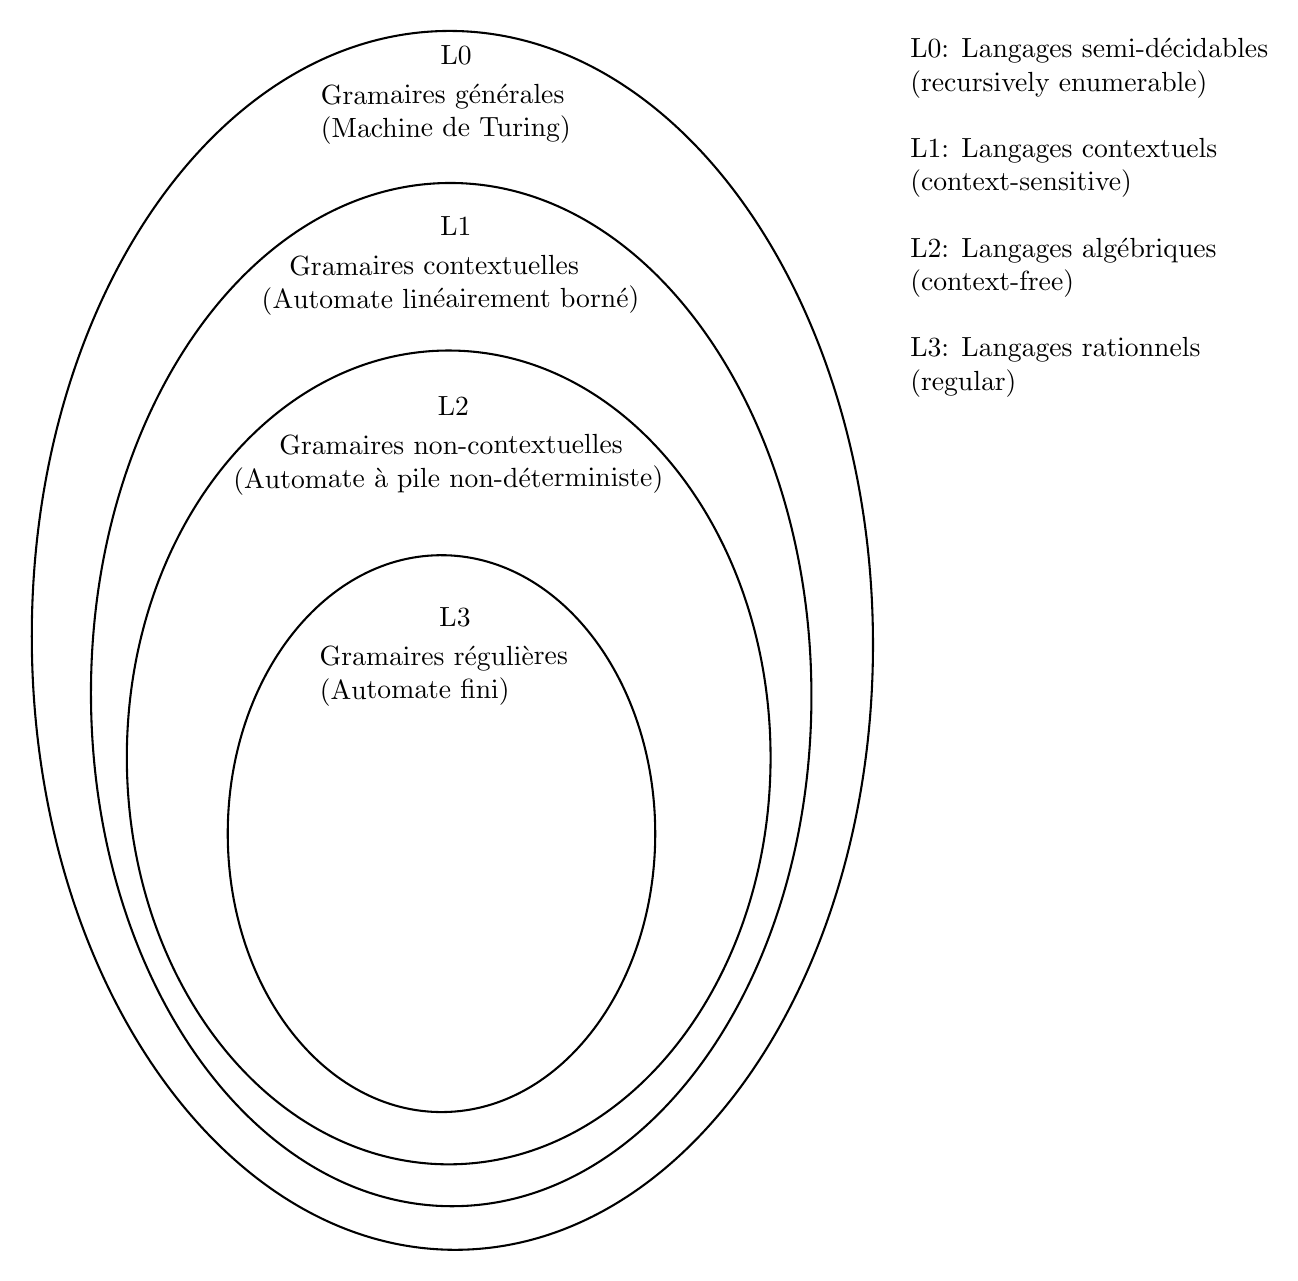
\begin{tikzpicture}[x=0.75pt,y=0.75pt,yscale=-1,xscale=1]
%uncomment if require: \path (0,777); %set diagram left start at 0, and has height of 777

%Shape: Ellipse [id:dp589513737865884]
\draw   (212.11,6.76) .. controls (324.01,5.68) and (415.95,136.27) .. (417.45,298.43) .. controls (418.95,460.59) and (329.45,592.92) .. (217.54,593.99) .. controls (105.63,595.07) and (13.7,464.48) .. (12.2,302.32) .. controls (10.7,140.16) and (100.2,7.83) .. (212.11,6.76) -- cycle ;
%Shape: Ellipse [id:dp20608648020649545]
\draw   (212.36,80.01) .. controls (308.21,78.91) and (386.76,188.37) .. (387.8,324.5) .. controls (388.85,460.63) and (311.99,571.88) .. (216.14,572.99) .. controls (120.29,574.09) and (41.75,464.63) .. (40.7,328.5) .. controls (39.66,192.37) and (116.51,81.11) .. (212.36,80.01) -- cycle ;
%Shape: Ellipse [id:dp9918973051483866]
\draw   (211.57,160.73) .. controls (297.22,159.72) and (367.3,246.68) .. (368.12,354.95) .. controls (368.93,463.22) and (300.16,551.8) .. (214.52,552.81) .. controls (128.88,553.81) and (58.79,466.85) .. (57.98,358.58) .. controls (57.16,250.31) and (125.93,161.73) .. (211.57,160.73) -- cycle ;
%Shape: Ellipse [id:dp8223736553004263]
\draw   (208.59,259.34) .. controls (265.47,258.67) and (312.01,318.18) .. (312.55,392.26) .. controls (313.1,466.35) and (267.43,526.96) .. (210.56,527.63) .. controls (153.69,528.31) and (107.14,468.8) .. (106.6,394.71) .. controls (106.05,320.62) and (151.72,260.02) .. (208.59,259.34) -- cycle ;

% Text Node
\draw (149.79,12.8) node [anchor=north west][inner sep=0.75pt]  [rotate=-359.73] [align=left] {\begin{minipage}[lt]{98.022pt}\setlength\topsep{0pt}
\begin{center}
L0
\end{center}
Gramaires générales\\(Machine de Turing)
\end{minipage}};
% Text Node
\draw (433.93,9) node [anchor=north west][inner sep=0.75pt]   [align=left] {L0: Langages semi-décidables\\(recursively enumerable)\\\\L1: Langages contextuels\\(context-sensitive)\\\\L2: Langages algébriques\\(context-free)\\\\L3: Langages rationnels\\(regular)};
% Text Node
\draw (121.26,95.32) node [anchor=north west][inner sep=0.75pt]  [rotate=-359.73] [align=left] {\begin{minipage}[lt]{140.57844pt}\setlength\topsep{0pt}
\begin{center}
L1
\end{center}
 \ \ \ Gramaires contextuelles\\(Automate linéairement borné)
\end{minipage}};
% Text Node
\draw (107.59,181.9) node [anchor=north west][inner sep=0.75pt]  [rotate=-359.73] [align=left] {\begin{minipage}[lt]{159.29000000000002pt}\setlength\topsep{0pt}
\begin{center}
L2
\end{center}
 \ \ \ \ \ Gramaires non-contextuelles\\ \ \ (Automate à pile non-déterministe)
\end{minipage}};
% Text Node
\draw (149.22,283.45) node [anchor=north west][inner sep=0.75pt]  [rotate=-359.73] [align=left] {\begin{minipage}[lt]{98.01044000000002pt}\setlength\topsep{0pt}
\begin{center}
L3
\end{center}
Gramaires régulières\\ \ \ \ (Automate fini)
\end{minipage}};


\end{tikzpicture}
